\documentclass[a4paper,11pt]{article}

\usepackage{amssymb}
\usepackage{amstext}
\usepackage{amsmath}
\usepackage{amsthm}
\usepackage{booktabs}
\usepackage{graphicx}
\usepackage{float}
\usepackage{url}

\usepackage{xcolor}
\newcommand{\bluenote}[1]{\color{blue}{ \em #1 }\color{black}}

\usepackage{geometry}
 \geometry{
 a4paper, %letterpaper,
 total={17cm,22.8cm},
 margin=24mm,
 top=22.4mm,
 bottom=25.4mm
 }
 
% Times new roman
\usepackage{mathptmx}

\usepackage[T1]{fontenc}

\thispagestyle{empty} 

\setlength{\parindent}{0pt}

% For comment boxes.
\usepackage[colorinlistoftodos,prependcaption,textsize=tiny]{todonotes}
\newcommand{\giselle}[1]{\todo[linecolor=red,backgroundcolor=red!25,bordercolor=red]{G: #1}}

\author{%
%  \fontsize{10}{12}\selectfont
  \begin{minipage}[t]{0.47\textwidth}
    \centering
    Samar Rahmouni \\ srahmoun@andrew.cmu.edu
  \end{minipage}
  \and
  %
  \begin{minipage}[t]{0.45\textwidth}
    \centering
    Advisor: Prof. Giselle Reis \\ giselle@cmu.edu
  \end{minipage}%
  \vspace*{2ex}
}


\date{}

\title{{\Large\sc Senior Thesis 2021-22\\[2ex]}{\LARGE\bf Mid-Semester Report\vspace*{3ex}}}


\begin{document}

\maketitle 

\section{Abstract}
\textcolor{red}{To redo, don't read.}
Reinforcement learning (RL), though a powerful and simple trial-and-error procedure that found a lot of success in games like Go, cannot be deployed in the real world 
because of the lack of security guarantees. For instance, though an autonomous car trained with reinforcement learning is bound to learn how to drive, the AI needs to crash 
to learn that crashing is not desirable. 

\medskip

In the context of the proposed thesis, we investigate both the security and the interpretability aspect of reinforcement learning in a cooperative adaptive cruise control inspired from \cite{vnc20},
in the aim of finding how formal security frameworks can guide the representation, robustness and extrapolation of knowledge in reinforcement
learning agents. We do so by experimenting and comparing both the optimization and security of three different RL implementations. 

\medskip

The first is a basic tabular Q-learning where we expect no security guarantees. The second is a hybrid architecture that incorporates the safe controller in \cite{vnc20} in a RL architecture. 
The safe controller (SC) computes a range of safe velocities given the current state of the environment in the car platooning scenario. Precisely, for multiple vehicles following each other, platooning aims to reduce the distance between them, hence taking less space on the road 
and allowing more vehicles to occupy highways, for instance. In the RL architecture, the SC then constricts the possible actions of the RL continuously at every given time step and the role of the RL is purely 
to find the optimal velocity in the safe range to minimize the distance between the cars. The third is what we will define as a logic-based inference RL. We investigate learning inferences rules in a deterministic environment 
where the result of an action given a state is not dependent on any probabilistic event. We approach the problem using inductive reasoning where the goal is to incorporate the learned rule knowledge into the decision making of a tabular Q-learning RL agent. 
In the given scenario, this will make use of the SC to develop a mapping from the state representation to a reward scheme, i.e. punish before a crash is bound to happen and adapt the Q-value and the epsilon-greedy approach. 

{\color{red}Writing rules (by Giselle Reis):
\begin{itemize}
  \item Each sentence must be a natural continuation of the next, reusing
  the same words and concepts. This ensures a natural reading flow.
  \item Crucial concepts are emphasized when they appear for the first
  time.
  \item Information is given in a \emph{by need} basis. Don't overload
  the reader with more information than necessary at any given point.
\end{itemize}
}

\section{Introduction}
Implementing a robust adaptive controller that is effective in terms
of precision, time\giselle{What does time effectiveness mean?}, and quality of decision
when facing dynamic and uncertain scenarios, has always been a central
challenge in AI and robotics.\giselle{This sentence is too long and I
think it has a lot of information. You need to explain what are each
of these measures and why they are challenging.}
As autonomous cars are deployed, IoT is popularized, and human-robot interactions become more complex, we
are more and more confronted with the need for robotic agents that can effectively and continually adapt
to their surroundings, not only in simulation, but also in practice, when deployed as a cyber-physical system. 
Since we are unable to provide a repertoire of all possible scenarios and actions,
our agents need to be able to autonomously predict and adapt to new
changes. RL\giselle{Reinforcement Learning (RL)} is an approach that
supports developing these capabilities\giselle{What capabilites? Be
explicit.}, \giselle{This should be another sentence.}it is also the solution that AlphaGo, Deepmind AlphaStar, and OpenAI Five have
adopted \cite{li2019reinforcement}, respectively for Go, StarCraft II and Dota 2 and found success in. 

However, as RL is a trial-and-error process, a car trained using RL is
bound to crash to learn not to crash again. Safe reinforcement
learning\giselle{Define what you mean by safe reinforcement learning.
Is it learning without error?} is then crucial 
to investigate in order to be able to deploy it in larger scale, but also out of simulation. 
The survey in \cite{kurdkelly2003} lays the foundations of
verifications goals for Artificial Neural Networks (ANNs) to be
ensured for safety-critical tasks\giselle{If this is relevant, explain
what these verification goals are.}. The need for this behavioral
constraints\giselle{What do you mean by behavioral constraints?} stems from the inability to analyze and 
describe the behavior of NNs.\giselle{I don't know what you mean with
the sentence that ends here.} The same argument translates to RL. In
general, reinforcement learning does not ensure any of the
verification conditions\giselle{Which are?} in \cite{kurdkelly2003}. 
The observable behavior of a RL agent is unpredictable\giselle{Why?}
(e.g. AlphaGo gamestyle) and will more often than not take hazardous
actions since it is a trial-and-error process. Hence, it is important
to investigate
the use of verified safety controller\giselle{What is a verified
safety controller?} and the interpretability of RL\giselle{From the
text above, it is not clear how interpretability plays a role.} in
order to achieve these verifications goals\giselle{Which are?}.  


\subsection{Reinforcement Learning as Trial-and-Error} 
Reinforcement Learning is a method of learning that maps situations to
actions in order to maximize its rewards
\cite{sutton2018reinforcement}.\giselle{This needs to be explained in
more detail. The reward function is the crucial measure for these
algorithms and this needs to be clear for a reader that is not
familiar with this field.} 
Compared to data-driven machine learning algorithms, reinforcement learning has the advantage of not requiring a prior dataset as the agent is not told what to do, but rather 
learns from the effect of its actions on the environment. Consider figure \ref{fig:rl}. 
\begin{figure}[H]
  \centering
  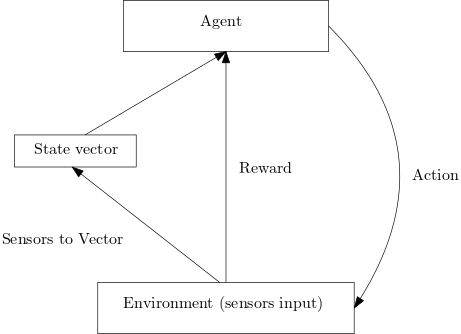
\includegraphics[scale=0.6]{rlroutine.png}
  \caption{Reinforcement Learning Routine}
  \label{fig:rl}
\end{figure}
The following RL routine shown in figure \ref{fig:rl} describes the high-level of how an agent using reinforcement learning can be trained. Precisely, 
given the current external observation, which in practice are based on the sensors output are used to construct a state vector. This distinction between state and observation 
is crucial in a RL setting. The underlying assumption of any RL
implementation is the \textbf{Markov Property}.\giselle{I don't see
how this is relevant to the explanation of how a RL algorithm works...} In other words, 
the current state provides enough information to predict the future state and its associated reward. This needs not to be deterministic. It's the idea that a decision that was made $n$ steps
in the past should not affect the current step the agent is in.
\textcolor{red}{add some notes how this actually works a lot in
practice.} Thus, it's only through the state vector that the agent is
trained.\giselle{This is not relevant at this point. See this
paragraph rewritten below.} 
At every timestep, the agent takes in the state vector, and chooses an action. The environment then rewards it accordingly.  

\medskip
{\color{red}G: Last paragraph rewritten, for example.}
\medskip

The diagram in Figure~\ref{fig:rl} is a high-level description of how
an agent using reinforcement learning can be trained.  
%
The lower box represents the \emph{environment} as seen by the agent
according to its sensors.
%
The current state of the environment is represented as a \emph{state
vector}.
%
At each iteration, the agent will receive the state vector as input,
and needs to choose an \emph{action} to take.
%
Once the action is taken, the environment is updated to the next state
and the agent receives a \emph{reward} as feedback.
%
This reward is a domain dependent function that represents how
``good'' the state is.
%
The agent's goal is to increase its reward by taking actions that
reach better states each time.\giselle{This last sentence is like a
magic box to me. Maybe we need to make it less magic, maybe not.}
%
This is achieved by ... {\color{red}Do we want to go there?}

\giselle{As a last paragraph in this section, emphasize how the reward
function is the crucial aspect of the RL algorithm. The better the
reward function, the faster the agent learns and with fewer errors.}

\subsection{Engineering issues with Reinforcement Learning}
\giselle{Why are these called engineering issues? Aren't they just
issues? It might be better to call them challenges though.}

In the routine shown in figure \ref{fig:rl}, we can identify
two\giselle{It looks like you mention more than two issues below.}
main engineering issues\giselle{challenges} that are raised once RL is chosen for
training.\giselle{The issues/challenges are from RL itself, not about
the figure. You don't need to mention it here.} First, in the case of
most scenarios\giselle{All scenarios need a reward function, so remove
this part between the commas.}, 
a reward function needs to be designed. There are reasonable criteria
on how this should be designed.\giselle{This is the place where you
should explain that the reward function is domain dependent, and a
function on the state vector. To make your case stronger, you need to
argue that sometimes it is intuitive, sometimes not. Give examples.} For instance, consider a reinforcement learning agent whose goal is to predict the weather. 
The closer the prediction\giselle{How do you know if the prediction is
close since it predicts the future?}, the more reward it should be given. \textcolor{red}{Add some references about how best rewards are chosen.}

\medskip

{\color{red}Add a paragraph explaining that this is a search problem
on a potentially infinite tree, and smart ways to prune this tree
result in more efficient learning. This tree pruning is done
indirectly by the reward function.}

\medskip

Second, there is a need to choose from the observation what we assume is needed for the state to hold the Markov Property. This can be easy to do for certain scenarios. 
For instance, \textcolor{red}{add an example here}. However, it becomes more complex as tasks require more sensing. For instance, consider an autonomous vehicle. The observation could be 
the current fuel, velocity, position, proximity sensors and camera feedback. It is a problem similar to feature extraction in most Machine Learning (ML) settings. \textcolor{red}{How it's usually being done in practice}
\giselle{I think we agreed to leave this out. It only complicates the
problem and it is not a problem you are proposing to solve in your
work.}


\medskip

\giselle{I think the next two paragraphs are not so relevant anymore.
What you can say is: if a RL algorithm runs into fewer error
situations, it is safer to be deployed in the real world. But as Prof.
Gianni mentioned, everything always starts with a simulation.}

The result of training is a policy, a function to map states to action, thus that maximizes the cumulative rewards. 
However, several problems come into place when considering the deployment of the trained agent. First, given the mapping from observation to state vector, 
certain uncertainties will not be expected, thus there can be no expectation on how the agent will behave. 
This results in an unsafe trained agent, thus constricting reinforcement learning to the realm of simulation. 

\medskip 

Simulation in itself poses multiple issues. The first is again, the need to design and account for how the external real-world environment would behave. 
This can be hard to do accurately, and usually is the more exhausting part of the implementation process. A best case scenario is to be able to train any agent using RL in the 
real-world. This can be done if we are able to guarantee some safety properties. Those safety properties need not to be perfect, but should severly decrease the possibility of accidents 
and dangerous outcomes. 

\subsection{Safety in Reinforcement Learning}

To be able to guarantee some safety properties, we look into a safe controller implementation that acts like an oracle, constricting the possible actions 
of the RL agent to those it deems "safe". The following work will focus on (1) the integration of this safe controller to 
the reinforcement learning training process, see section \ref{rlscarchitecture} and (2) the theoretical guarantees of the safe controller and its implementation, see section \ref{scspecs} and finally, (3) testing the hybrid architecture of RL+SC 
on a vehicle platooning problem done in simulation as to compare its safety and optimality with a basic RL implementation.
Figure \ref{fig:overviewsol} is an overview of the proposed solution and the high level basis of the work. 

\begin{figure}[H]
  \centering
  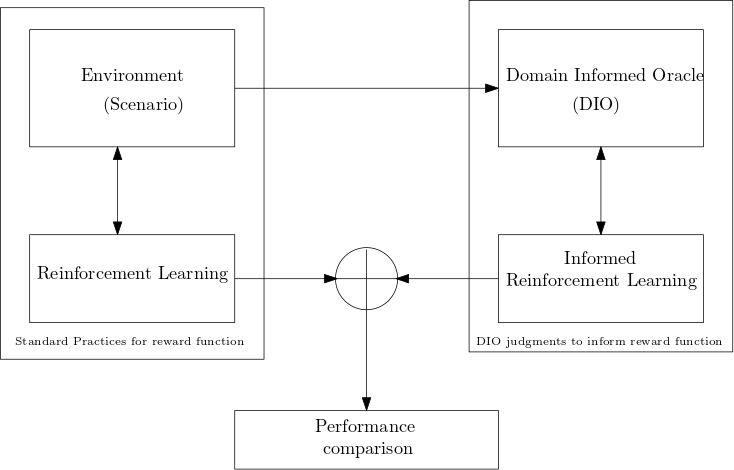
\includegraphics[scale=0.6]{overview.png}
  \caption{Overview of the proposed solution}
  \label{fig:overviewsol}
\end{figure}

Note that (3) is a work in progress. The current formalization of the scenario for the problem of vehicle platooning 
and its significance is in section \ref{vehicleplat}.


\section{RL+SC Architecture} \label{rlscarchitecture}
Assume for the following that there exists a safe controller (SC) type of oracle that is able to take in the current
environment as observed by the reinforcement learning agent and decide deterministically on a set of possible safe actions. 
More on the practical specifications of this safe controller can be found in section \ref{scspecs}. 
We suppose that the SC can output false positives but never false negatives. In other words, if a safe controller deems 
a situation safe, then it has to be safe. We allow it to misjudge a situation and be conservative on safety. 

\medskip 

\begin{figure}[H]
  \centering
  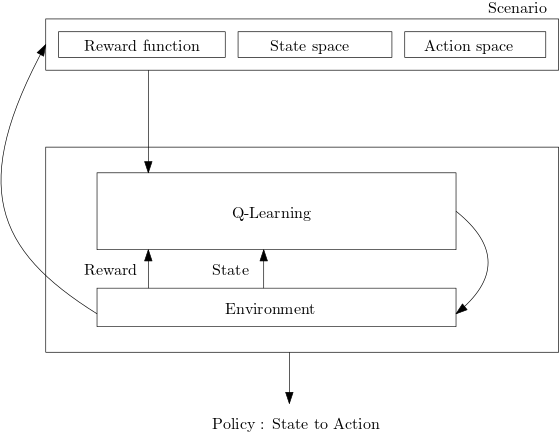
\includegraphics[scale=0.55]{basicrl.png}
  \caption{Basic reinforcement learning architecture}
  \label{fig:basicrl}
\end{figure}


\begin{figure}[H]
  \centering
  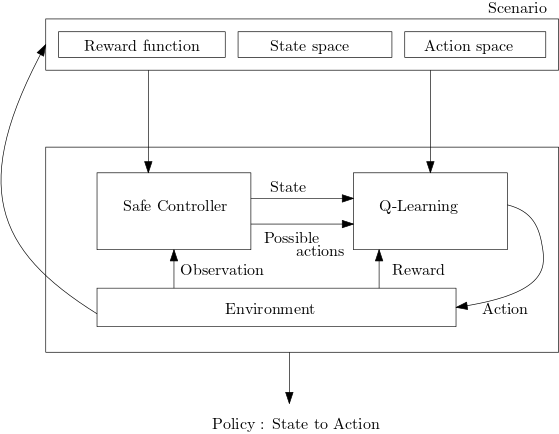
\includegraphics[scale=0.55]{rlsc.png}
  \caption{Safe controller integrated in reinforcement learning architecture}
  \label{fig:scinrl}
\end{figure}

\section{Safe Controller Specifications} 
\label{scspecs}
\giselle{Oracle Specification (possible new title if DIO is not yet
defined)}

In the previous section, we assume the existence of a safe controller that acts like an oracle.
In our setting the safe controller takes in the current observation of the environment and 
returns the state representation and a set of possible actions to the reinforcement learning side.
\giselle{This changed. The DIO receives a state as input and outputs
an evaluation about that state. This evaluation could be a number
between 0 and 1 or a discrete value. Decide what you are going to use
and explain that. You can mention other possible measures, but make it
clear which one you will use because the implementation of a correct
DIO -- for any domain -- relies on it.}
Some conditions need to hold on both the state representation and the set of possible actions to define a 'good' safe controller.
In the following section, we lay down the foundations 
for such a module, starting by the guarantees we would like for it to have. 

\begin{enumerate}
  \item The returned state upholds the Markov Property.
  \item The resulting state of any action of the possible set of actions 
        should not include any known fatality conditions, except if necessary. 
\end{enumerate}
\giselle{I think this no longer applies, since DIO does not return
states. Instead you need to explain what a domain expert user needs to
do to integrate their prolog program into the RL framework. Namely:
(1) output the values as you have selected before (number in a range
or discrete set of values); and (2) have a translation from state
vectors to ground facts.}

We make the following assumptions, (1) actions are deterministic, meaning if an agent chooses to go left, they will go left with certainty, 
(2) sensors can be faulty and they obey a gaussian distribution for their uncertainty, (3) the world is filled with uncertainties and the safe controller cannot account 
for all of them. Note that in the following, we will define uncertainty as an evolution of the world given the sensors that is unknown by the safe controller, i.e.
no known step semantics for the uncertain.
\giselle{This also no longer applies. The prolog program can take
uncertainty into account based on specific knowledge of the domain and
sensors. It is advisable I suppose, but it depends on the programmer.}

\medskip 


Given our assumptions, we make those first observations. \newline
\textbf{Observation 1:} Though our SC cannot account for all uncertainties, there exists a set of expected information that is informed 
given known step semantics, i.e. $E_t$. Precisely, considering actions are deterministic and the problem is a Markov Decision Problem (MDP), the SC can compute the resulting expected state. \newline
\textbf{Observation 2:} The SC cannot ensure that the expected will be the next observed. \newline
\giselle{I think these observations would now be different. DIO can
have the knowledge of actions and can simulate a couple of steps ahead
to predict the near future. The more DIO can simulate, the more
precise is its feedback to the agent. A simple DIO is made up only of
judgments about states. A smarter DIO simulates the rules of the game
and take a few steps before judging.}

\textbf{Observation 3:} Since there is a finite number of sensors,
every sensor output can be defined as a proposition associated with a
specific value. \newline
\giselle{That would be an intuitive way to translate state vectors
into facts, but not the only one. This depends on the domain.}

\medskip 

By taking our observation 1 and our assumption 2, we can construct the following deterministic approach to compute the state and the set of possible actions. 


\begin{figure}[H]
  \centering
  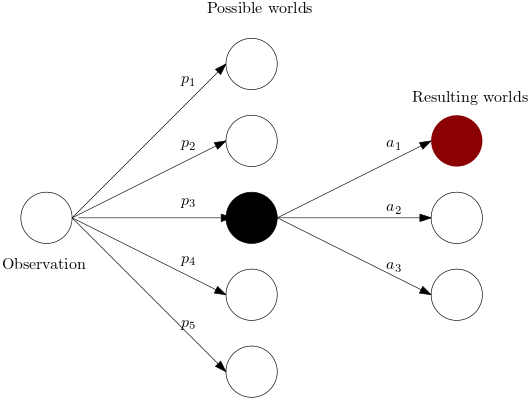
\includegraphics[scale=0.55]{scworlds.png}
  \caption{SC to compute the state and possible actions}
  \label{fig:scworld}
\end{figure}
\giselle{This is the game tree simulated by a good DIO :) }

In the first layer, if we know the distribution of our sensors, we are able to compute the possible worlds and assume the one with the highest probability.
In the case of figure \ref{fig:scworld}, it is $p_5$. By assuming our state and the possible actions, we can utilize domain specific knowledge into 
computing the expected possible worlds. Given some fatality conditions, it is possible to assess whether a given world is desirable or should be blocked. 

\textcolor{blue}{There's a lot more than can go on here. A couple of my notes.}
\begin{itemize}
  \item Consider history, basically : $[S_t, a, S_{t+1}/E_t]$. We are technically able to compute the level of uncertainty of a result, since
        we're only dealing with numerical computation. Basically, suppose I never had $sound(e)$ in my observation, I don't know what it is, for all I know, 
        it could be the worse possible outcome and I have no clue how to react to it. I should be able then to choose my safest action, the one I know to always result 
        in non fatal conditions. Suppose I survive such an uncertainty, then now I know what the next state was actually compared to what I expected,
        if I 'normalize' the next state while accounting for uncertainty of sensors and compare it to my expected, I now have a numerical value that 
        I can embed in my step semantics to adapt for this uncertainty. Inductive reasoning basically. 
  \item Obviously, the more domain specific knowledge, the less uncertainties to deal with.
  \item Could also just give the uncertainty decision to the RL, basically randomly try it. It's a sacrifice we're willing to make 
        for learning. We're still ensuring some aspect of safety so already doing better.
  \item For a better argument on how the deployment in real life can be fine is a distinction between 
        undesirable vs fatal. I don't really want to swerve into the road but I also won't exist if I crash into a car. 
\end{itemize}

\subsection{From SC to verification conditions} 
\textcolor{red}{todo.}
 

\section{Vehicle Platooning : Case Study} \label{vehicleplat}
To put our approach in practice, we consider the case of vehicle platooning. The setting is as follows: multiple autonomous vehicles 
are tasked with following each other while ensuring that they minimize the gap between them. 
As described in \cite{LarssonErik2015Tvpp}, forming a vehicle platoon helps reduce fuel consumption severly. The closer the proximity and faster the speed, the more fuel is saved. 
Even by assuming no faulty communication between the vehicles, the uncertainties of the road make it a challenge to deploy autonomous vehicles trained using reinforcement learning 
with that goal in mind. For instance, consider an unexpected construction on the usual route that the vehicles take. 
As the leader of the platoon will be the first to notice, we would like to communicate as early as possible to the followers that a decelaration needs to happen. 
In the context of reinforcement learning, there are two cases, (1) the agents have been trained on that occurence, thus they all decrease their velocities, or 
(2) the agents have never encountered that problem in training, thus are bound to fail. 

\medskip 


\subsection{Preliminary Results}
\textcolor{red}{todo}
\subsection{Discussion}
\textcolor{red}{todo}

\section{Related Work}
One of the many ways safety has been approached is by formalization and symbolic reasoning. 
In the case of artificial intelligence, recent work proposes neurosymbolic integration. 
Neurosymbolic integration has been an ongoing work in the last years towards a combination of deep learning (DL) and symbolic reasoning.
The work has been a response to criticism of DL, precisely, the lack of formal semantics and intuitive explanation and the lack of expert knowledge towards guiding machine learning models. 
Key questions the field targets are identifying the necessary and sufficient building blocks of AI \cite{garcez2020neurosymbolic}, namely, how can we provide the semantics of knowledge, 
and work towards meta-learning? Meta-learning in reinforcement learning is the problem of learning-to-learn, which is about efficiently
adapting a learned policy to conditions and tasks that were not encountered in the past. In RL, meta-learning
involves adapting the learning parameters, balancing exploration and exploitation to direct the
agent interaction \cite{gupta_meta-reinforcement_2018,schweighofer_meta-learning_2003}. Meta-learning is a central problem in AI, since an agent that can solve more
and more problems it has not seen before, approaches the ideal of a general-purpose AI. 

\medskip

Approaches that were concerned with safe reinforcement learning, have approached the problem in previous work \cite{Garca2015ACS} in two ways. First was changing the optimization criteria \cite{rockafellar2000}, precisely by incorporating risk into the performance of the policy.
Namely, either considering the worst case scenario and constraining on it, reducing the variance to be more sensitive or applying constraints i.e. only update the policy if the action is in a safe set. 
This does not however guarantee safety, but tends to minimize the probability of risk, hence not allowing RL systems to be deployed in the physical world. 
Second was to consider the exploration process, either by incorporating external knowledge i.e. learning from demonstration \cite{Siebel2007EvolutionaryRL} or adopting a risk directed exploration \cite{law2005}. These approaches can be considered rigid, 
as requiring more data and expert knowledge that needs to be proven safe and sound, or in the latter, decreasing the efficiency and requiring more time for the learning process. 
In particular, in these previous two approaches, work that makes use of formal security frameworks is yet to be investigated. 

\medskip

Some of the more recent work that does investigate a hybrid architecture (i.e. RL and symbolic reasoning) makes use of
set-theoretic techniques and constraint satisfaction problems to optimize from the constraints \cite{Li2021SafeRL}, or proposes a reactive system called a shield \cite{alshiekh2017} to either constraint the actions given by the environment or adapt them once the RL module chooses one. 
In both cases, the added safety controller is described by its specifications, rather than being an independent existing controller. 

\medskip

\textcolor{red}{Partially observable Markov decision process belief system to improve from observation to state vector.}

\medskip

\textcolor{red}{Explain how this idea is novel.}

\section{Conclusions}
\textcolor{red}{todo.}

\newpage

\bibliographystyle{unsrt}
\bibliography{biblio.bib}



\end{document}
